\newpage



\section{Experiments}
\label{sec:verify}


\subsection{Datasets}

The dataset that were considered for the experiments are  CIFAR10 \cite{CIFAR}, CIFAR100- 20 \cite{CIFAR} STL10 \cite{yao2016automatic} and ImageNet \cite{ImageNet}.

%
%\begin{figure}[!htbp]
%\begin{center}
%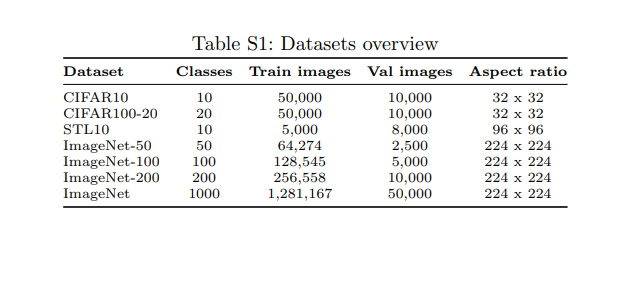
\includegraphics[width=6in]{6.PNG}
%\end{center}
%\end{figure}
%

%%%%%%%%%%%%%%%%%%%%%%%%%%%%%%%%%%

\setlength{\tabcolsep}{4pt}
\begin{table}[ht!]
\scriptsize
\begin{center}
\caption{Datasets overview}
\label{tab: datasets}
\begin{tabular}{@{}l cccc @{}}
\toprule
\textbf{Dataset} & \textbf{Classes} & \textbf{Train images} & \textbf{Val images} & \textbf{Aspect ratio}\\ 
\midrule
CIFAR10 & 10 & 50,000 & 10,000 & 32 x 32\\
CIFAR100-20 & 20 & 50,000 & 10,000 & 32 x 32\\
STL10 & 10 & 5,000 & 8,000 & 96 x 96\\
ImageNet-50 & 50 & 64,274 & 2,500 & 224 x 224\\
ImageNet-100 & 100 & 128,545 & 5,000 & 224 x 224\\
ImageNet-200 & 200 & 256,558 & 10,000 & 224 x 224\\
ImageNet & 1000 & 1,281,167 & 50,000 & 224 x 224\\
\bottomrule
\end{tabular}
\end{center}
\end{table}

%%%%%%%%%%%%%%%%%%%%%%%%%%%%%%%%%%

\subsection{Training setup}

The training was done on standard ResNet-18 backbone with batch size 128 and in the fine tuning step with threshold of 0.99 and using Adam optimizer. For every sample, the 20 nearest neighbors are determined through an instance discrimination task based on noise contrastive estimation (NCE) \cite{gutmann2010noise}  and SimCLR \cite{chen2020improved} implementation for the instance discrimination task on the dataset and MoCo \cite{chen2020simple} on ImageNet.


\subsection{Validation criterion} 

The model based on the lowest loss was selected as the best model during the clustering step.
For the self-labeling step, Based on the number of confident samples the model’s weights were saved.



\subsection{Augmentations} 

The authors were able to get better results using strong augmentations during the training. 
RandAugment \cite{cubuk2020randaugment}, followed by Cutout \cite{devries2017improved} for the augmentation part and it was composed of four randomly selected transformations.

\newpage

\subsection{Ablation studies} 
An ablation study studies the performance of an AI system by removing certain components, to understand the contribution of the component to the overall system. The term is by analogy with biology (removal of components of an organism), and, continuing the analogy, is particularly used in the analysis of artificial neural nets, by analogy with ablative brain surgery.\cite{DBLP:journals/corr/abs-1901-08644}



%%%% ABLATION METHOD TABLE %%%
%\setlength{\tabcolsep}{4pt}
%\begin{table}[t]
%\begin{minipage}[t]{0.5\linewidth}
%\scriptsize
%\begin{center}
%\caption{Ablation Method CIFAR10}
%\label{table:ablation_method}
%\begin{tabular}{lcc}
%\toprule
%\textbf{Setup} & \ \textbf{ACC} \\
% &  (Avg $\pm$ Std) \\
%\midrule
%Pretext + K-means & $65.9\pm5.7$ \\
%%Sample + Batch Entropy Loss & $19.2\pm0.9$ \\
%%SCAN-Loss (Standard Augs) (Ours)& $62.7\pm3.3$ \\
%SCAN-Loss (SimCLR) & $78.7\pm1.7$ \\
%\hspace{0.1in} (1) Self-Labeling (SimCLR) & $10.0\pm0$ \\
%\hspace{0.1in} (2) Self-Labeling (RA) & $87.4\pm1.6$ \\
%SCAN-Loss (RA) & $81.8\pm1.7$ \\
%\hspace{0.1in} (1) Self-Labeling (RA) & $87.6\pm0.4$ \\
%\bottomrule
%\end{tabular}
%\end{center}
%\end{minipage}
%\hspace*{\fill}
%\begin{minipage}[t]{0.5\linewidth}
%\scriptsize
%\begin{center}
%\caption{Ablation Pretext CIFAR10}
%\label{table: ablation_pretext}
%\begin{tabular}{lcc}
%\toprule
%\textbf{Pretext Task} & \textbf{Clustering}& \textbf{ACC}\\
%  & & (Avg $\pm$ Std)  \\
%\midrule
%RotNet~\cite{RotNet}  & K-means & $27.1\pm2.1$ \\
%  & SCAN & $74.3\pm3.9$ \\
%%Feature Decoupling~\cite{feng2019self} & $83.0\pm3.4$\\
%Inst. discr.~\cite{wu2018unsupervised} & K-means & $52.0\pm4.6$\\
% & SCAN &  $83.5\pm4.1$\\
%Inst. discr.~\cite{chen2020simple} & K-means & $65.9\pm5.7$ \\
% & SCAN &  $87.6\pm0.4$\\
%\bottomrule
%\end{tabular}
%\end{center}
%\end{minipage}
%\end{table}
%\setlength{\tabcolsep}{1.4pt}


%
\begin{figure}[!htbp]
\begin{center}
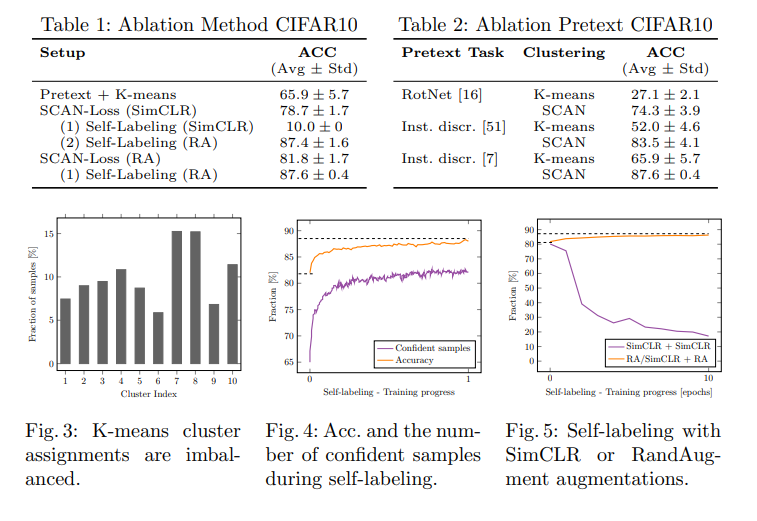
\includegraphics[width=6in]{8.PNG}
\end{center}
\end{figure}

\FloatBarrier

\medskip

The paper presented the performance gains through an ablation study on CIFAR10.



Some observation to be noted, K-means clustering with NCE pretext features results in an accuracy of 65.9\%. Interestingly, applying K-means to the pretext features outperforms prior state-of-the-art methods for unsupervised classification based on end-to-end learning schemes. This observation supports the paper's primary claim of the benefit of separating clustering and feature learning.

Applying image augmentation to both the samples and their mined neighbors also improves the performance (78.7\% vs. 81.8\%). During self-labeling, the network slowly becomes more confident and therefore fine-tuning the network enhances the quality of the clustering(81.8\% to 87.6\%). 


